\documentclass[a4paper, 12pt]{article}
\usepackage[a4paper,top=1.5cm, bottom=1.5cm, left=1cm, right=1cm]{geometry}

% Работа с русским языком
\usepackage[utf8]{inputenc}
\usepackage{mathtext}                % русские буквы в формулах
\usepackage[english, russian]{babel} % локализация и переносы

\usepackage{graphicx}   % Вставка изображений
\usepackage{float}      % "Плавающие" изображения3
\usepackage{wrapfig}    % Обтекание фигур (таблиц, картинок и прочего)
\usepackage{subfig}
\graphicspath{ {./images/} }

\usepackage{tabularx}
\usepackage{multirow}
\usepackage{amsmath}
\usepackage{amsfonts}
\usepackage{indentfirst}
\usepackage{longtable}
\graphicspath{{pictures/}}
\usepackage[square,sort,comma,numbers]{natbib}
\usepackage{bm}

%%% Колонтитулы
\usepackage{titleps}
\newpagestyle{main}{
	\setheadrule{0.4pt}
	\sethead{Резонанс напряжений в последовательном контуре}{}{}
	\setfootrule{0.4pt}                       
	\setfoot{ФРКТ МФТИ, 2023}{}{\thepage} 
}
\pagestyle{main}  

\begin{document}
    \begin{titlepage}
	\begin{center}
            {\large МОСКОВСКИЙ ФИЗИКО-ТЕХНИЧЕСКИЙ ИНСТИТУТ (НАЦИОНАЛЬНЫЙ ИССЛЕДОВАТЕЛЬСКИЙ УНИВЕРСИТЕТ)}
	\end{center}
 
	\begin{center}
		{\large Физтех-школа радиотехники и компьютерных технологий}
	\end{center}
	
	\vspace{8cm}
	{\LARGE
		\begin{center}
                {\bf Отчёт о выполнении лабораторной работы 3.2.2}\\
                Резонанс напряжений в последовательном контуре
		\end{center}
	}
	\vspace{5cm}
	\begin{flushright}
		{\Large Автор:\\ Тихонов Дмитрий Романович, \\
			\vspace{0.2cm}
			студент группы Б01-206}
	\end{flushright}
	\vspace{5cm}
	\begin{center}
		\Large Долгопрудный, 2023
	\end{center}
    \end{titlepage}


    \section{Введение}

    \noindent \textbf{Цель работы:} исследование резонанса напряжений в последовательном колебательном контуре с изменяемой ёмкостью, получение амплитудно-частотных и фазово-частотных характеристик, определение основных параметров контура. \\

    \noindent \textbf{В работе используются:} генератор сигналов, источник напряжения, нагрузкой которого является последовательный колебательный контур с переменной ёмкостью, двухканальный осциллограф, цифровые вольтметры.
    
    \section{Теоретические сведения и методика измерений}

    \subsection{Описание установки, вывод основных соотношений}

    Схема экспериментального стенда для изучения резонанса напряжений в последовательном колебательном контуре показана на рисунке \ref{installation}. Синусоидальный сигнал от генератора GFG-8255A поступает через согласующую RC-цепочку на вход источника напряжения, собранного на операционном усилителе \textit{ОУ}. Питание операционного усилителя осуществляется встроенным блоком-выпрямителем от сети переменного тока $220$ Вольт (цепь питания на схеме не показана). Источник напряжения, обладающий по определению нулевым внутренним сопротивлением, фактически обеспечивает с высокой точностью постоянство амплитуды сигнала на меняющейся по величине нагрузке –- последовательном колебательном контуре, изображенном на рисунке в виде эквивалентной схемы.

    \begin{figure}[H]
        \centering
        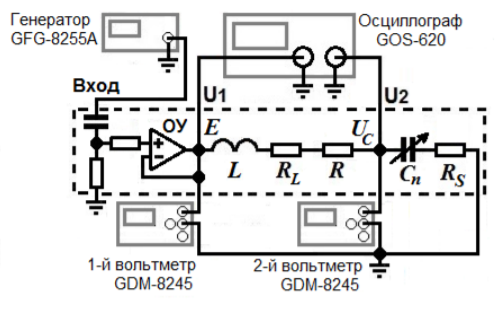
\includegraphics{images/installation.png}
        \caption{Схема экспериментального стенда}
        \label{installation}
    \end{figure}

    Катушка индуктивности $L$ на ферритовом каркасе обладает малым сопротивлением по постоянному току и высокой собственной резонансной частотой $f_r \geq 1,3$ МГц. В общем случае каждая катушка, помимо индуктивности $L$, характеризуется также собственной ёмкостью $C_L$ и активным сопротивлением потерь $R_L$, распределёнными по её длине. Принимается, что эти величины сосредоточены в отдельных элементах схемы, образующих с индуктивностью $L$ замкнутую колебательную цепь с собственной резонансной частотой 
    
    \begin{equation}
        \label{freq}
        f_r = \frac{1}{2 \pi \sqrt{L C}}.
    \end{equation} 
    
    Вследствие влияния ёмкости $C_L$ при измерении на частоте $f$ \textit{эффективное} определяется значение индуктивности $L_{eff} = L/(1-f^2/f_r^2)$, которое может заметно отличаться от истинной величины $L$. В рабочем диапазоне частот нашего контура выполняется неравенство $f \ll f_r$, так что в эквивалентной схеме контура на рис. \ref{installation} индуктивность представлена истинным значением $L$ и активным сопротивлением $R_L$.

    Оценим возможные активные потери в конденсаторах, воспользовавшись представлением конденсатора с ёмкостью $C$ последовательной эквивалентной схемой с \textit{эквивалентным последовательным сопротивлением}

    \begin{equation}
        R_S = \frac{U_{RS}}{I} = \frac{U_{RS}}{\omega C U_{CS}} = \frac{1}{\omega C} \tg \delta.
    \end{equation}

    В колебательный контур нашей установки входит резистор $R$, снижающий его добротность. Это сделано для упрощения получения и обработки резонансных кривых. Таким образом, суммарное активное сопротивление контура принимается равным

    \begin{equation}
        R_\Sigma = R + R_L + R_S.
    \end{equation}

    Далее будем пользоваться методом комплексных амплитуд. Для импедансов индуктивности $Z_L$, ёмкости $Z_C$ и последовательного контура $Z = Z_L + R + Z_C$:

    \begin{equation}
        \label{impedance}
        Z_L = R_L + i\omega L, \hspace{4mm} Z_C = R_S - i\frac{1}{\omega C}, \hspace{4mm} Z = R_\Sigma + i \left( \omega L - \frac{1}{\omega C} \right).
    \end{equation}

    Комплексные амплитуды тока в контуре $\bm{I} = \bm{\mathcal{E}}/Z$ и напряжений индуктивности $\bm{U}_L = Z_L \bm{I}$ и ёмеости $\bm{U}_C = Z_C \bm{I}$ при нулевой начальной фазе $\varphi_0$ напряжения на контуре $\bm{\mathcal{E}} = \mathcal{E} e^{i \varphi_0}$ удобно представить в виде

    \begin{equation}
        \bm{I} = \frac{\mathcal{E}}{R_\Sigma} \frac{1}{1+iQ \left( \frac{\omega}{\omega_0} - \frac{\omega_0}{\omega} \right)}, \hspace{4mm} \bm{U}_L = i\mathcal{E}Q \frac{\omega}{\omega_0}\frac{1-i R_L/\rho}{1+ iQ \left( \frac{\omega}{\omega_0} - \frac{\omega_0}{\omega} \right)}, \hspace{4mm} \bm{U}_C = -i\mathcal{E}Q \frac{\omega_0}{\omega}\frac{1+i \tg{\delta}}{1 + iQ \left( \frac{\omega}{\omega_0} - \frac{\omega_0}{\omega} \right)},
        \label{eq:complex_1}
    \end{equation}

    где $\omega_0 = 1/\sqrt{LC}$ -- резонансная частота, определяемая из условия $\operatorname{Im} Z = 0$, то есть из условия действительности контура, $\rho = \sqrt{L/C}$ -- \textit{реактивное}, или \textit{волновое}, сопротивление контура, $Q$ -- добротность колебательного контура.

    \begin{equation}
        \label{qual}
        Q = \frac{\rho}{R_\Sigma} = \frac{\omega_0 L}{R_\Sigma} = \frac{1}{\omega_0 C R_\Sigma} \gg 1.
    \end{equation}

    Рассмотрим случай, когда $\lvert \Delta \omega \rvert \ll \omega_0$, тогда мы можем упростить соотношения \ref{eq:complex_1} и представить их в виде

    \begin{equation}
        \label{Ires}
        \bm{I} = \frac{\mathcal{E}}{R_\Sigma} \frac{e^{i\varphi_I}}{\sqrt{1 + (\tau \Delta \omega )^2}}, \hspace{4mm} \varphi_I = -\arctg (\tau \Delta \omega ), 
    \end{equation}

    \begin{equation}
        \label{Ures_C}
        \bm{U}_C = \mathcal{E}Q \frac{\omega_0}{\omega} \frac{e^{i \varphi_C}}{\sqrt{1 + (\tau \Delta \omega )^2}}, \hspace{4mm} \varphi_C = -\frac{\pi}{2} + \delta - \arctg (\tau \Delta \omega),
    \end{equation}

    \begin{equation}
        \label{Ures_L}
        \bm{U}_L = \mathcal{E}Q \frac{\omega_0}{\omega} \frac{e^{i \varphi_L}}{\sqrt{1 + (\tau \Delta \omega )^2}}, \hspace{4mm} \varphi_L = \frac{\pi}{2} - \frac{R_L}{\rho} - \arctg (\tau \Delta \omega),
    \end{equation}

    где $\tau = 2L/R_\Sigma = 2Q/\omega_0$ -- \textit{время релаксации}, $\gamma = 1/\tau$ -- \textit{коэффициент затухания}. В выражениях (\ref{Ures_C}) и (\ref{Ures_L}) мы пренебрегли относительными поправками порядка $Q^{-2}$, а величину $\delta$ сохранили для общности, положив её константой. Из формул (\ref{Ires}), (\ref{Ures_C}) и (\ref{Ures_L}) видно, что зависимости модулей тока $\bm{I}$ в контуре и напряжений $\bm{U}_L$ на индуктивности и $\bm{U}_C$ на ёмкости от частоты $\omega$ внешней ЭДС имеют вблизи резонанса практически одинаковый характер.

    При резонансе, когда $\omega = \omega_0$, $\Delta \omega = 0$, выражения для модулей комплексных амплитуд и их фаз:

    \begin{equation}
        I(\omega_0) = \frac{\mathcal{E}}{R_\Sigma}, \hspace{4mm} \varphi_I(\omega_0) = 0,
    \end{equation}

    \begin{equation}
        U_L(\omega_0) = Q\mathcal{E}, \hspace{4mm} \varphi_L(\omega_0) = \frac{\pi}{2} - \frac{R_L}{\rho},
    \end{equation}

    \begin{equation}
        \label{resc}
        U_C(\omega_0) = Q\mathcal{E}, \hspace{4mm} \varphi_C(\omega_0) = -\frac{\pi}{2} + \delta.
    \end{equation}

    \subsection{Расчётные формулы}

    Зная резонансную частоту (\eqref{freq}) можно найти индуктивность катушки
    
    \begin{equation}
    \label{induct}
        L = \frac{1}{4 \pi ^2 C f^2}.
    \end{equation}
    
     Из формулы \eqref{qual}, или из формулы $ \rho = \sqrt{L/C} $ можно найти реактивное сопротивление контура. 
     
     Зная суммарное активное сопротивление $R_\Sigma$ и $R_S = 10^{-3} \rho$, можно найти $R_L$ -- активное сопротивление катушки. 
     
     Для определения добротности контура $Q$ применяется формула \eqref{resc}.
     
     Сопротивление $R_\Sigma$ найдём из формулы \eqref{qual}.
     
     При исследовании АЧХ, будем использовать формулу
    
    \begin{equation}
        \label{ACHH}
        Q = \frac{\omega_0}{\delta \omega},
    \end{equation}
    
    где $ \delta \omega $ -- ширина резонансной кривой на уровне $ U_C (\omega_0) / \sqrt{2} $.
    
    При исследовании ФЧХ применим формулу (\ref{Ures_C}), согласно которой расстояние по оси $\omega$ между точками, в которых фаза $\varphi_C$ меняется от $-\pi /4$ до $-3 \pi / 4$, равно $2 / \tau$, где $\tau$ -- время релаксации.
    
    \section{Результаты измерений и обработка данных}

    \subsection{Резонансные параметры контуров}
    \label{respar}
    
    В результате измерения резонансных частот и соответствующих им напряжений были получены данные, которые представлены в таблице \ref{tab:res_1}.

     \begin{figure}[H]
	\centering
	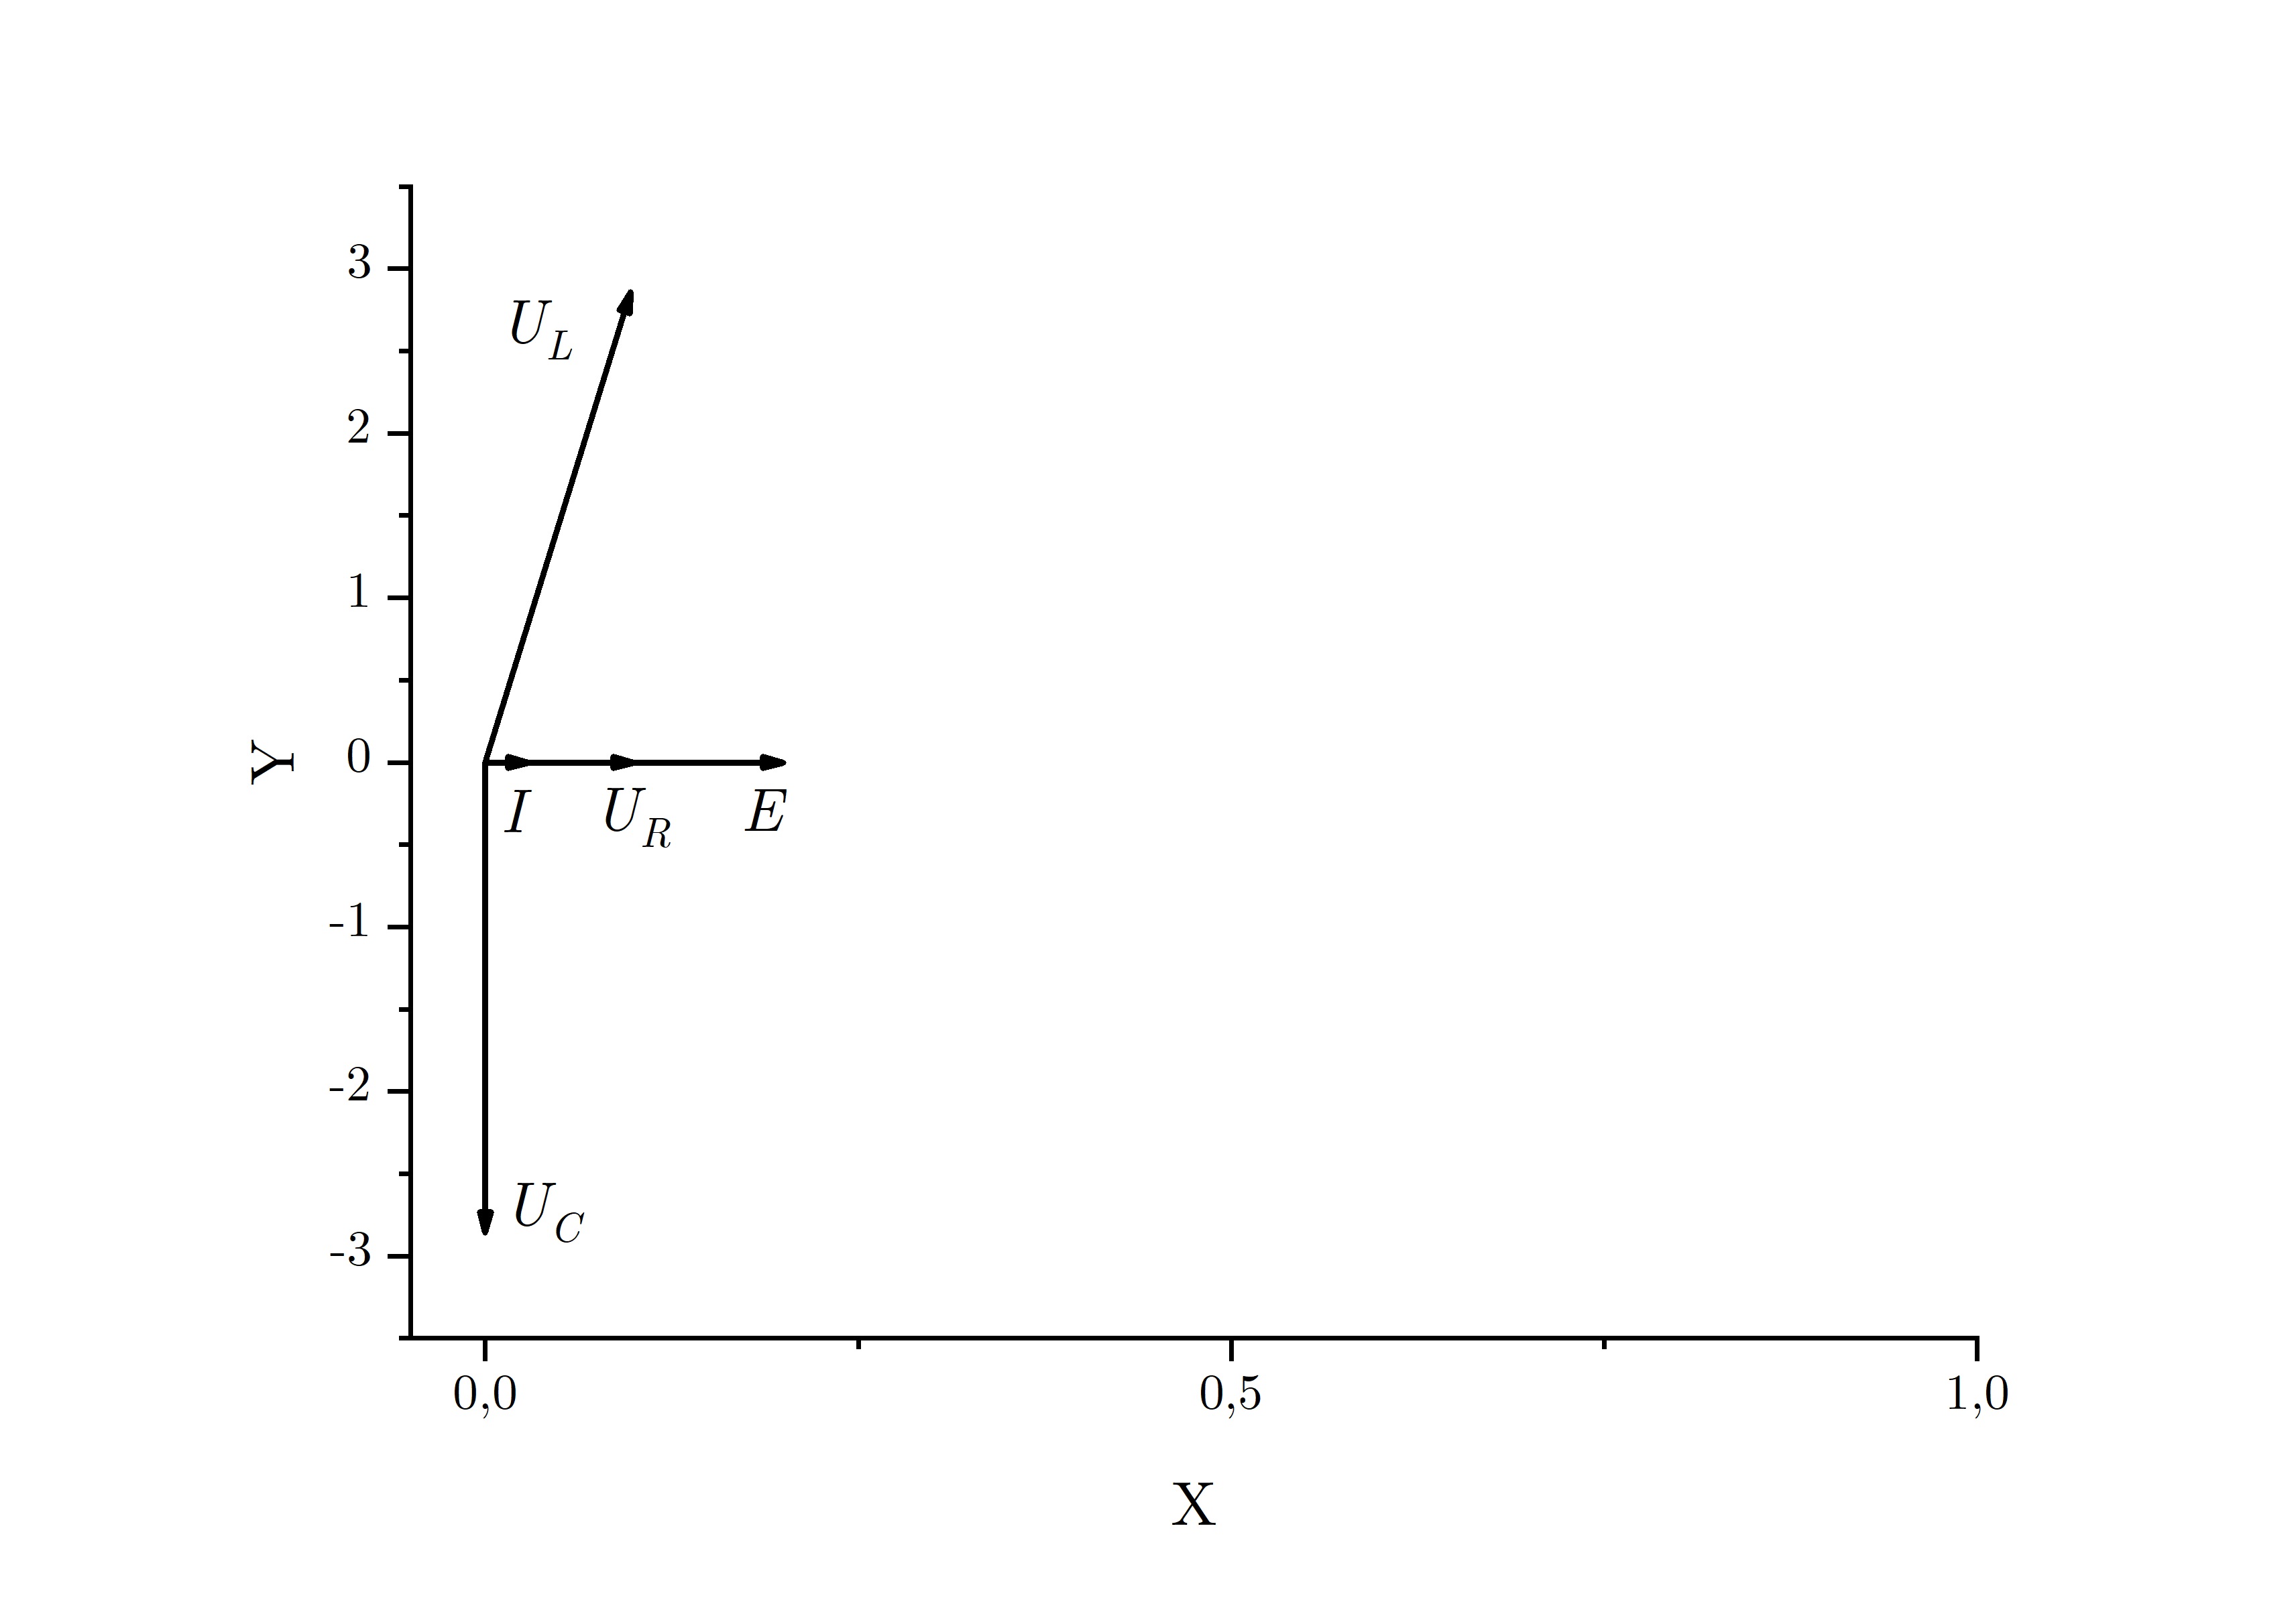
\includegraphics[height=0.4\textheight]{images/vec_diag.png}
	\caption{Векторная диаграмма для контура $C_n = 102,8$ нФ при $\mathcal{E} = 0,2$ В}
	\label{diag}
    \end{figure}

    \begin{table}[H]
        \centering
        \begin{tabular}{|ccccccccccc|}
        \hline
        \multicolumn{1}{|c|}{$C_n$, нФ} & \multicolumn{1}{c|}{$f_{0n}$, кГц} & \multicolumn{1}{c|}{$U_C$, В} & \multicolumn{1}{c|}{$\mathcal{E}$, В} & \multicolumn{1}{c|}{$L$, мкГн} & \multicolumn{1}{c|}{$Q$} & \multicolumn{1}{c|}{$\rho$, Ом} & \multicolumn{1}{c|}{$R_\Sigma$, Ом} & \multicolumn{1}{c|}{$R_S$, Ом} & \multicolumn{1}{c|}{$R_L$, Ом} & $I$, мА \\ \hline
        \multicolumn{1}{|c|}{24,8} & \multicolumn{1}{c|}{32,447} & \multicolumn{1}{c|}{5,059} & \multicolumn{1}{c|}{0,2009} & \multicolumn{1}{c|}{970} & \multicolumn{1}{c|}{25,2} & \multicolumn{1}{c|}{197,79} & \multicolumn{1}{c|}{7,85} & \multicolumn{1}{c|}{0,198} & \multicolumn{1}{c|}{4,2} & 25,6 \\ \hline
        \multicolumn{1}{|c|}{33,2} & \multicolumn{1}{c|}{28,031} & \multicolumn{1}{c|}{4,529} & \multicolumn{1}{c|}{0,2007} & \multicolumn{1}{c|}{971} & \multicolumn{1}{c|}{22,6} & \multicolumn{1}{c|}{171,02} & \multicolumn{1}{c|}{7,58} & \multicolumn{1}{c|}{0,171} & \multicolumn{1}{c|}{3,9} & 26,5 \\ \hline
        \multicolumn{1}{|c|}{47,6} & \multicolumn{1}{c|}{23,384} & \multicolumn{1}{c|}{3,936} & \multicolumn{1}{c|}{0,2006} & \multicolumn{1}{c|}{973} & \multicolumn{1}{c|}{19,6} & \multicolumn{1}{c|}{142,99} & \multicolumn{1}{c|}{7,29} & \multicolumn{1}{c|}{0,143} & \multicolumn{1}{c|}{3,6} & 27,5 \\ \hline
        \multicolumn{1}{|c|}{57,5} & \multicolumn{1}{c|}{21,337} & \multicolumn{1}{c|}{3,571} & \multicolumn{1}{c|}{0,2006} & \multicolumn{1}{c|}{968} & \multicolumn{1}{c|}{17,8} & \multicolumn{1}{c|}{129,72} & \multicolumn{1}{c|}{7,29} & \multicolumn{1}{c|}{0,130} & \multicolumn{1}{c|}{3,7} & 27,5 \\ \hline
        \multicolumn{1}{|c|}{68,0} & \multicolumn{1}{c|}{19,584} & \multicolumn{1}{c|}{3,423} & \multicolumn{1}{c|}{0,2005} & \multicolumn{1}{c|}{971} & \multicolumn{1}{c|}{17,1} & \multicolumn{1}{c|}{119,51} & \multicolumn{1}{c|}{7,00} & \multicolumn{1}{c|}{0,120} & \multicolumn{1}{c|}{3,4} & 28,6 \\ \hline
        \multicolumn{1}{|c|}{102,8} & \multicolumn{1}{c|}{15,989} & \multicolumn{1}{c|}{2,879} & \multicolumn{1}{c|}{0,2005} & \multicolumn{1}{c|}{964} & \multicolumn{1}{c|}{14,4} & \multicolumn{1}{c|}{96,83} & \multicolumn{1}{c|}{6,74} & \multicolumn{1}{c|}{0,097} & \multicolumn{1}{c|}{3,1} & 29,7 \\ \hline
        \multicolumn{4}{|c|}{Среднее значение} & \multicolumn{1}{c|}{970} & \multicolumn{4}{c|}{\multirow{4}{*}{}} & \multicolumn{1}{c|}{3,6} & \multirow{4}{*}{} \\ \cline{1-5} \cline{10-10}
        \multicolumn{4}{|c|}{СКП} & \multicolumn{1}{c|}{1,4} & \multicolumn{4}{c|}{} & \multicolumn{1}{c|}{0,1} &  \\ \cline{1-5} \cline{10-10}
        \multicolumn{4}{|c|}{Коэффициент Стьюдента} & \multicolumn{1}{c|}{2,6} & \multicolumn{4}{c|}{} & \multicolumn{1}{c|}{2,6} &  \\ \cline{1-5} \cline{10-10}
        \multicolumn{4}{|c|}{Случайная погрешность} & \multicolumn{1}{c|}{3,5} & \multicolumn{4}{c|}{} & \multicolumn{1}{c|}{0,4} &  \\ \hline
        \multicolumn{11}{c}{} \\ \hline
        \multicolumn{1}{|c|}{$C_n$, нФ} & \multicolumn{1}{c|}{$f_{0n}$, кГц} & \multicolumn{1}{c|}{$U_C$, В} & \multicolumn{1}{c|}{$\mathcal{E}$, В} & \multicolumn{1}{c|}{$L$, мкГн} & \multicolumn{1}{c|}{$Q$} & \multicolumn{1}{c|}{$\rho$, Ом} & \multicolumn{1}{c|}{$R_\Sigma$, Ом} & \multicolumn{1}{c|}{$R_S$, Ом} & \multicolumn{1}{c|}{$R_L$, Ом} & $I$, мА \\ \hline
        \multicolumn{1}{|c|}{24,8} & \multicolumn{1}{c|}{32,305} & \multicolumn{1}{c|}{3,762} & \multicolumn{1}{c|}{0,1496} & \multicolumn{1}{c|}{979} & \multicolumn{1}{c|}{25,1} & \multicolumn{1}{c|}{198,65} & \multicolumn{1}{c|}{7,90} & \multicolumn{1}{c|}{0,199} & \multicolumn{1}{c|}{4,2} & 18,9 \\ \hline
        \multicolumn{1}{|c|}{33,2} & \multicolumn{1}{c|}{27,820} & \multicolumn{1}{c|}{3,355} & \multicolumn{1}{c|}{0,1495} & \multicolumn{1}{c|}{986} & \multicolumn{1}{c|}{22,4} & \multicolumn{1}{c|}{172,32} & \multicolumn{1}{c|}{7,68} & \multicolumn{1}{c|}{0,172} & \multicolumn{1}{c|}{4,0} & 19,5 \\ \hline
        \multicolumn{1}{|c|}{47,6} & \multicolumn{1}{c|}{23,275} & \multicolumn{1}{c|}{2,884} & \multicolumn{1}{c|}{0,1495} & \multicolumn{1}{c|}{982} & \multicolumn{1}{c|}{19,3} & \multicolumn{1}{c|}{143,66} & \multicolumn{1}{c|}{7,45} & \multicolumn{1}{c|}{0,144} & \multicolumn{1}{c|}{3,8} & 20,1 \\ \hline
        \multicolumn{1}{|c|}{57,5} & \multicolumn{1}{c|}{21,234} & \multicolumn{1}{c|}{2,650} & \multicolumn{1}{c|}{0,1494} & \multicolumn{1}{c|}{977} & \multicolumn{1}{c|}{17,7} & \multicolumn{1}{c|}{130,35} & \multicolumn{1}{c|}{7,35} & \multicolumn{1}{c|}{0,130} & \multicolumn{1}{c|}{3,7} & 20,3 \\ \hline
        \multicolumn{1}{|c|}{68,0} & \multicolumn{1}{c|}{19,548} & \multicolumn{1}{c|}{2,451} & \multicolumn{1}{c|}{0,1493} & \multicolumn{1}{c|}{975} & \multicolumn{1}{c|}{16,4} & \multicolumn{1}{c|}{119,73} & \multicolumn{1}{c|}{7,29} & \multicolumn{1}{c|}{0,120} & \multicolumn{1}{c|}{3,7} & 20,5 \\ \hline
        \multicolumn{1}{|c|}{102,8} & \multicolumn{1}{c|}{15,915} & \multicolumn{1}{c|}{2,050} & \multicolumn{1}{c|}{0,1493} & \multicolumn{1}{c|}{973} & \multicolumn{1}{c|}{13,7} & \multicolumn{1}{c|}{97,28} & \multicolumn{1}{c|}{7,08} & \multicolumn{1}{c|}{0,097} & \multicolumn{1}{c|}{3,5} & 21,1 \\ \hline
        \multicolumn{4}{|c|}{Среднее значение} & \multicolumn{1}{c|}{979} & \multicolumn{4}{c|}{\multirow{4}{*}{}} & \multicolumn{1}{c|}{3,8} & \multirow{4}{*}{} \\ \cline{1-5} \cline{10-10}
        \multicolumn{4}{|c|}{СКП} & \multicolumn{1}{c|}{2,0} & \multicolumn{4}{c|}{} & \multicolumn{1}{c|}{0,1} &  \\ \cline{1-5} \cline{10-10}
        \multicolumn{4}{|c|}{Коэффициент Стьюдента} & \multicolumn{1}{c|}{2,6} & \multicolumn{4}{c|}{} & \multicolumn{1}{c|}{2,6} &  \\ \cline{1-5} \cline{10-10}
        \multicolumn{4}{|c|}{Случайная погрешность} & \multicolumn{1}{c|}{5,1} & \multicolumn{4}{c|}{} & \multicolumn{1}{c|}{0,3} &  \\ \hline
        \multicolumn{11}{c}{} \\ \hline
        \multicolumn{1}{|c|}{$C_n$, нФ} & \multicolumn{1}{c|}{$f_{0n}$, кГц} & \multicolumn{1}{c|}{$U_C$, В} & \multicolumn{1}{c|}{$\mathcal{E}$, В} & \multicolumn{1}{c|}{$L$, мкГн} & \multicolumn{1}{c|}{$Q$} & \multicolumn{1}{c|}{$\rho$, Ом} & \multicolumn{1}{c|}{$R_\Sigma$, Ом} & \multicolumn{1}{c|}{$R_S$, Ом} & \multicolumn{1}{c|}{$R_L$, Ом} & $I$, мА \\ \hline
        \multicolumn{1}{|c|}{24,8} & \multicolumn{1}{c|}{32,071} & \multicolumn{1}{c|}{7,468} & \multicolumn{1}{c|}{0,3028} & \multicolumn{1}{c|}{993} & \multicolumn{1}{c|}{24,7} & \multicolumn{1}{c|}{200,10} & \multicolumn{1}{c|}{8,11} & \multicolumn{1}{c|}{0,200} & \multicolumn{1}{c|}{4,4} & 37,3 \\ \hline
        \multicolumn{1}{|c|}{33,2} & \multicolumn{1}{c|}{27,621} & \multicolumn{1}{c|}{6,611} & \multicolumn{1}{c|}{0,3028} & \multicolumn{1}{c|}{1000} & \multicolumn{1}{c|}{21,8} & \multicolumn{1}{c|}{173,56} & \multicolumn{1}{c|}{7,95} & \multicolumn{1}{c|}{0,174} & \multicolumn{1}{c|}{4,3} & 38,1 \\ \hline
        \multicolumn{1}{|c|}{47,6} & \multicolumn{1}{c|}{23,162} & \multicolumn{1}{c|}{5,763} & \multicolumn{1}{c|}{0,3028} & \multicolumn{1}{c|}{992} & \multicolumn{1}{c|}{19,0} & \multicolumn{1}{c|}{144,36} & \multicolumn{1}{c|}{7,58} & \multicolumn{1}{c|}{0,144} & \multicolumn{1}{c|}{3,9} & 39,9 \\ \hline
        \multicolumn{1}{|c|}{57,5} & \multicolumn{1}{c|}{21,018} & \multicolumn{1}{c|}{5,300} & \multicolumn{1}{c|}{0,3027} & \multicolumn{1}{c|}{997} & \multicolumn{1}{c|}{17,5} & \multicolumn{1}{c|}{131,69} & \multicolumn{1}{c|}{7,52} & \multicolumn{1}{c|}{0,132} & \multicolumn{1}{c|}{3,9} & 40,2 \\ \hline
        \multicolumn{1}{|c|}{68,0} & \multicolumn{1}{c|}{19,544} & \multicolumn{1}{c|}{4,697} & \multicolumn{1}{c|}{0,3026} & \multicolumn{1}{c|}{975} & \multicolumn{1}{c|}{15,5} & \multicolumn{1}{c|}{119,76} & \multicolumn{1}{c|}{7,72} & \multicolumn{1}{c|}{0,120} & \multicolumn{1}{c|}{4,1} & 39,2 \\ \hline
        \multicolumn{1}{|c|}{102,8} & \multicolumn{1}{c|}{15,767} & \multicolumn{1}{c|}{4,114} & \multicolumn{1}{c|}{0,3026} & \multicolumn{1}{c|}{991} & \multicolumn{1}{c|}{13,6} & \multicolumn{1}{c|}{98,19} & \multicolumn{1}{c|}{7,22} & \multicolumn{1}{c|}{0,098} & \multicolumn{1}{c|}{3,6} & 41,9 \\ \hline
        \multicolumn{4}{|c|}{Среднее значение} & \multicolumn{1}{c|}{991} & \multicolumn{4}{c|}{\multirow{4}{*}{}} & \multicolumn{1}{c|}{4,0} & \multirow{4}{*}{} \\ \cline{1-5} \cline{10-10}
        \multicolumn{4}{|c|}{СКП} & \multicolumn{1}{c|}{3,5} & \multicolumn{4}{c|}{} & \multicolumn{1}{c|}{0,1} &  \\ \cline{1-5} \cline{10-10}
        \multicolumn{4}{|c|}{Коэффициент Стьюдента} & \multicolumn{1}{c|}{2,6} & \multicolumn{4}{c|}{} & \multicolumn{1}{c|}{2,6} &  \\ \cline{1-5} \cline{10-10}
        \multicolumn{4}{|c|}{Случайная погрешность} & \multicolumn{1}{c|}{9,2} & \multicolumn{4}{c|}{} & \multicolumn{1}{c|}{0,3} &  \\ \hline
        \end{tabular}
        \caption{Результаты измерений}
        \label{tab:res_1}
    \end{table}

    Построим векторную диаграмму на рис. \ref{diag}, отложив $\mathcal{E}$ по оси абсцисс с масштабом в 2 раза больше, чем по оси ординат. Заметим, что согласно закону Кирхгофа
    
    \begin{equation}
        \label{kir}
	\mathcal{E} = U_R + U_С + U_L,
    \end{equation} 
    
    на диаграмме должно быть представлено равенство вектора $\mathcal{E}$ и суммы остальных трёх векторов.

    С помощью таблицы \ref{tab:res_1} был построен график $R_L(f_0) $ на рис. \ref{graph_RL}. Видно, что сопротивление меняется практически линейно. Можно предположить, что изменения связаны с потерями на перемагничивание сердечника катушки. 

    \begin{figure}[H]
        \centering
        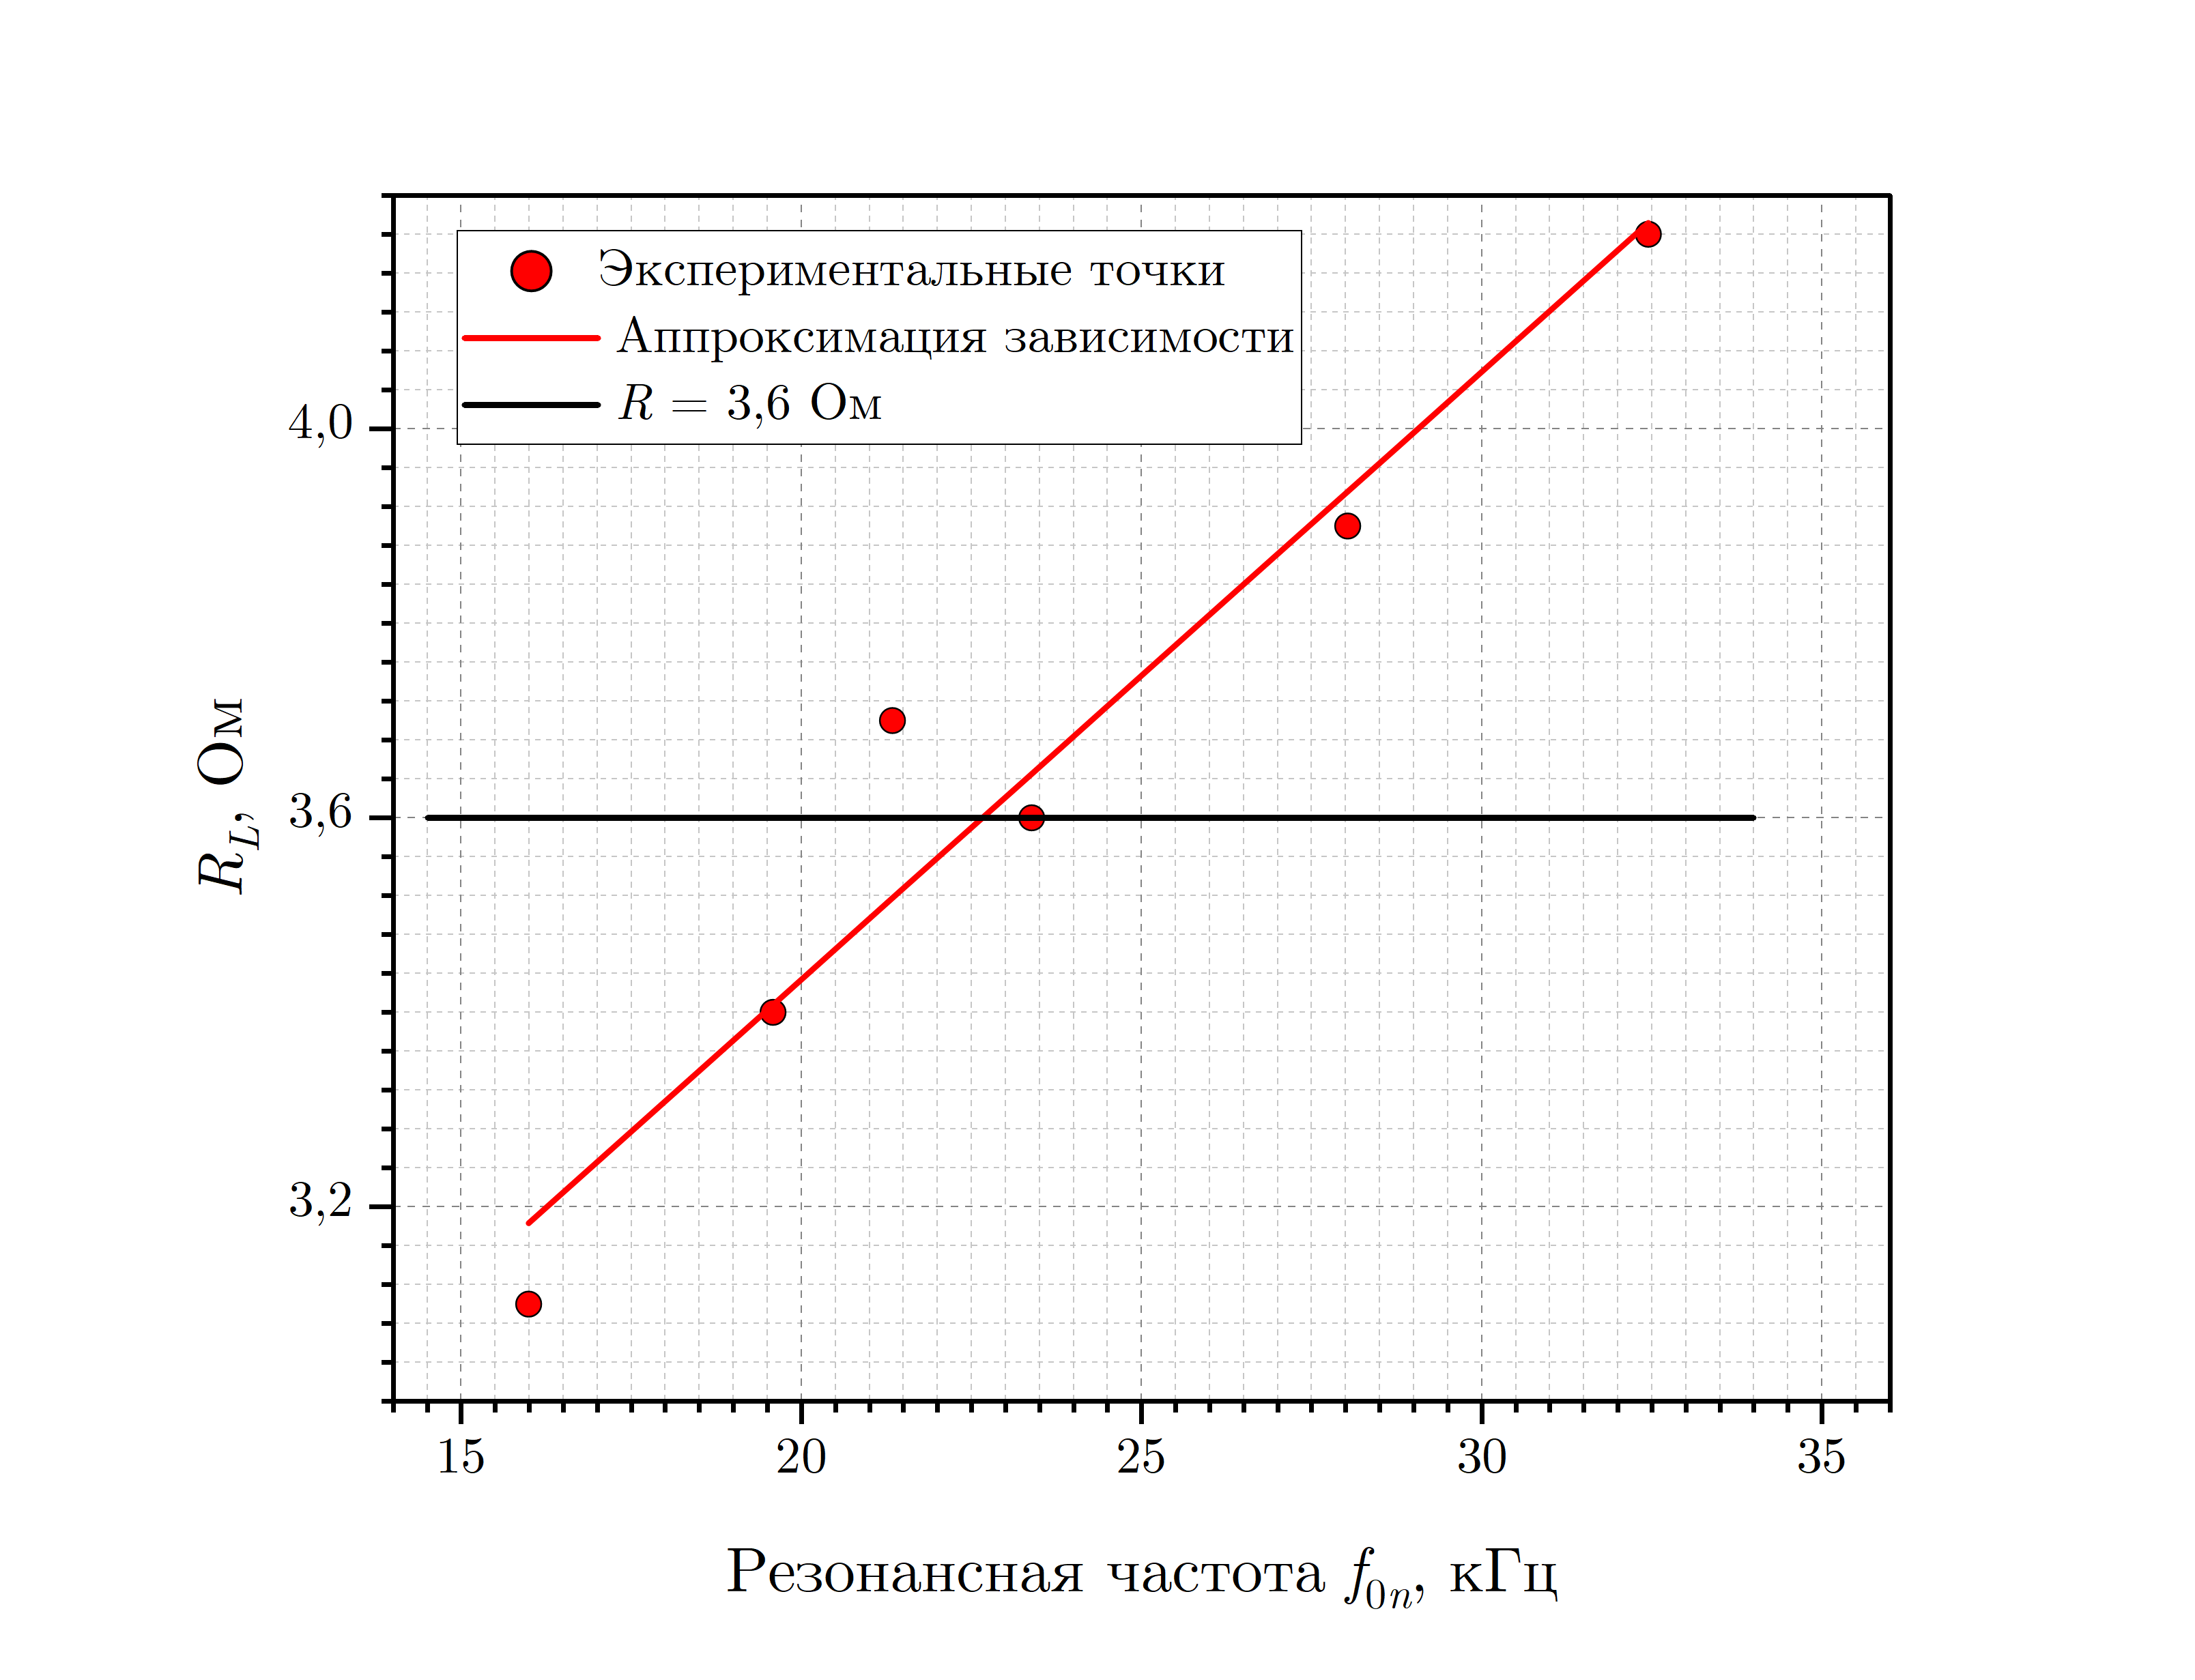
\includegraphics[width = 14 cm]{images/graph_RL.png}
        \caption{График изменения активного сопротивления индуктивности}
        \label{graph_RL}
    \end{figure}
    
    \subsection{Исследование АЧХ}

    Для контуров с двумя разными ёмкостями были сняты амплитудно-частотные характеристики $U_C(f)$. Результаты исследования данной зависимости приведены в таблице \ref{tab:res_AFC}.

    \begin{table}[H]
        \centering
        \begin{tabular}{|c|c|c|c|c|c|c|c|c|c|c|}
        \cline{1-5} \cline{7-11}
        $C_n$, нФ & $f$, Гц & $U_C$, В & $f/f_0$ & $U/U_0$ & \multirow{17}{*}{} & $C_n$, нФ & $f$, Гц & $U_C$, В & $f/f_0$ & $U/U_0$ \\ \cline{1-5} \cline{7-11} 
        \multirow{16}{*}{47,6} & 22459 & 2,291 & 0,9662 & 0,5825 &  & \multirow{16}{*}{68,0} & 18774 & 2,010 & 0,9615 & 0,5929 \\ \cline{2-5} \cline{8-11} 
         & 22471 & 2,314 & 0,9667 & 0,5884 &  &  & 18844 & 2,152 & 0,9651 & 0,6348 \\ \cline{2-5} \cline{8-11} 
         & 22520 & 2,404 & 0,9688 & 0,6112 &  &  & 18937 & 2,343 & 0,9698 & 0,6912 \\ \cline{2-5} \cline{8-11} 
         & 22658 & 2,729 & 0,9748 & 0,6939 &  &  & 19025 & 2,542 & 0,9743 & 0,7499 \\ \cline{2-5} \cline{8-11} 
         & 22846 & 3,236 & 0,9828 & 0,8228 &  &  & 19113 & 2,754 & 0,9789 & 0,8124 \\ \cline{2-5} \cline{8-11} 
         & 22949 & 3,505 & 0,9873 & 0,8912 &  &  & 19239 & 3,042 & 0,9853 & 0,8974 \\ \cline{2-5} \cline{8-11} 
         & 23050 & 3,731 & 0,9916 & 0,9486 &  &  & 19369 & 3,268 & 0,9920 & 0,9640 \\ \cline{2-5} \cline{8-11} 
         & 23245 & 3,933 & 1,0000 & 1,0000 &  &  & 19526 & 3,390 & 1,0000 & 1,0000 \\ \cline{2-5} \cline{8-11} 
         & 23300 & 3,865 & 1,0024 & 0,9827 &  &  & 19666 & 3,239 & 1,0072 & 0,9555 \\ \cline{2-5} \cline{8-11} 
         & 23468 & 3,631 & 1,0096 & 0,9232 &  &  & 19734 & 3,138 & 1,0107 & 0,9257 \\ \cline{2-5} \cline{8-11} 
         & 23616 & 3,326 & 1,0160 & 0,8457 &  &  & 19851 & 2,922 & 1,0166 & 0,8620 \\ \cline{2-5} \cline{8-11} 
         & 23719 & 3,101 & 1,0204 & 0,7885 &  &  & 19981 & 2,664 & 1,0233 & 0,7858 \\ \cline{2-5} \cline{8-11} 
         & 23818 & 2,885 & 1,0247 & 0,7335 &  &  & 20086 & 2,455 & 1,0287 & 0,7242 \\ \cline{2-5} \cline{8-11} 
         & 24000 & 2,503 & 1,0325 & 0,6364 &  &  & 20193 & 2,258 & 1,0342 & 0,6661 \\ \cline{2-5} \cline{8-11} 
         & 24080 & 2,365 & 1,0359 & 0,6013 &  &  & 20280 & 2,108 & 1,0386 & 0,6218 \\ \cline{2-5} \cline{8-11} 
         & 24182 & 2,185 & 1,0403 & 0,5556 &  &  & 20332 & 2,024 & 1,0413 & 0,5971 \\ \cline{1-5} \cline{7-11}
        \end{tabular}
        \caption{Результаты измерения зависимости амплитудно-частотных характеристик}
        \label{tab:res_AFC}
    \end{table}

    По таблице \ref{tab:res_AFC} на одном графике были построены амплитудно-частотные характеристики в координатах $f, U_C(f)$ для выбранных контуров (рис. \ref{graph_AFC}).

    \begin{figure}[H]
        \centering
        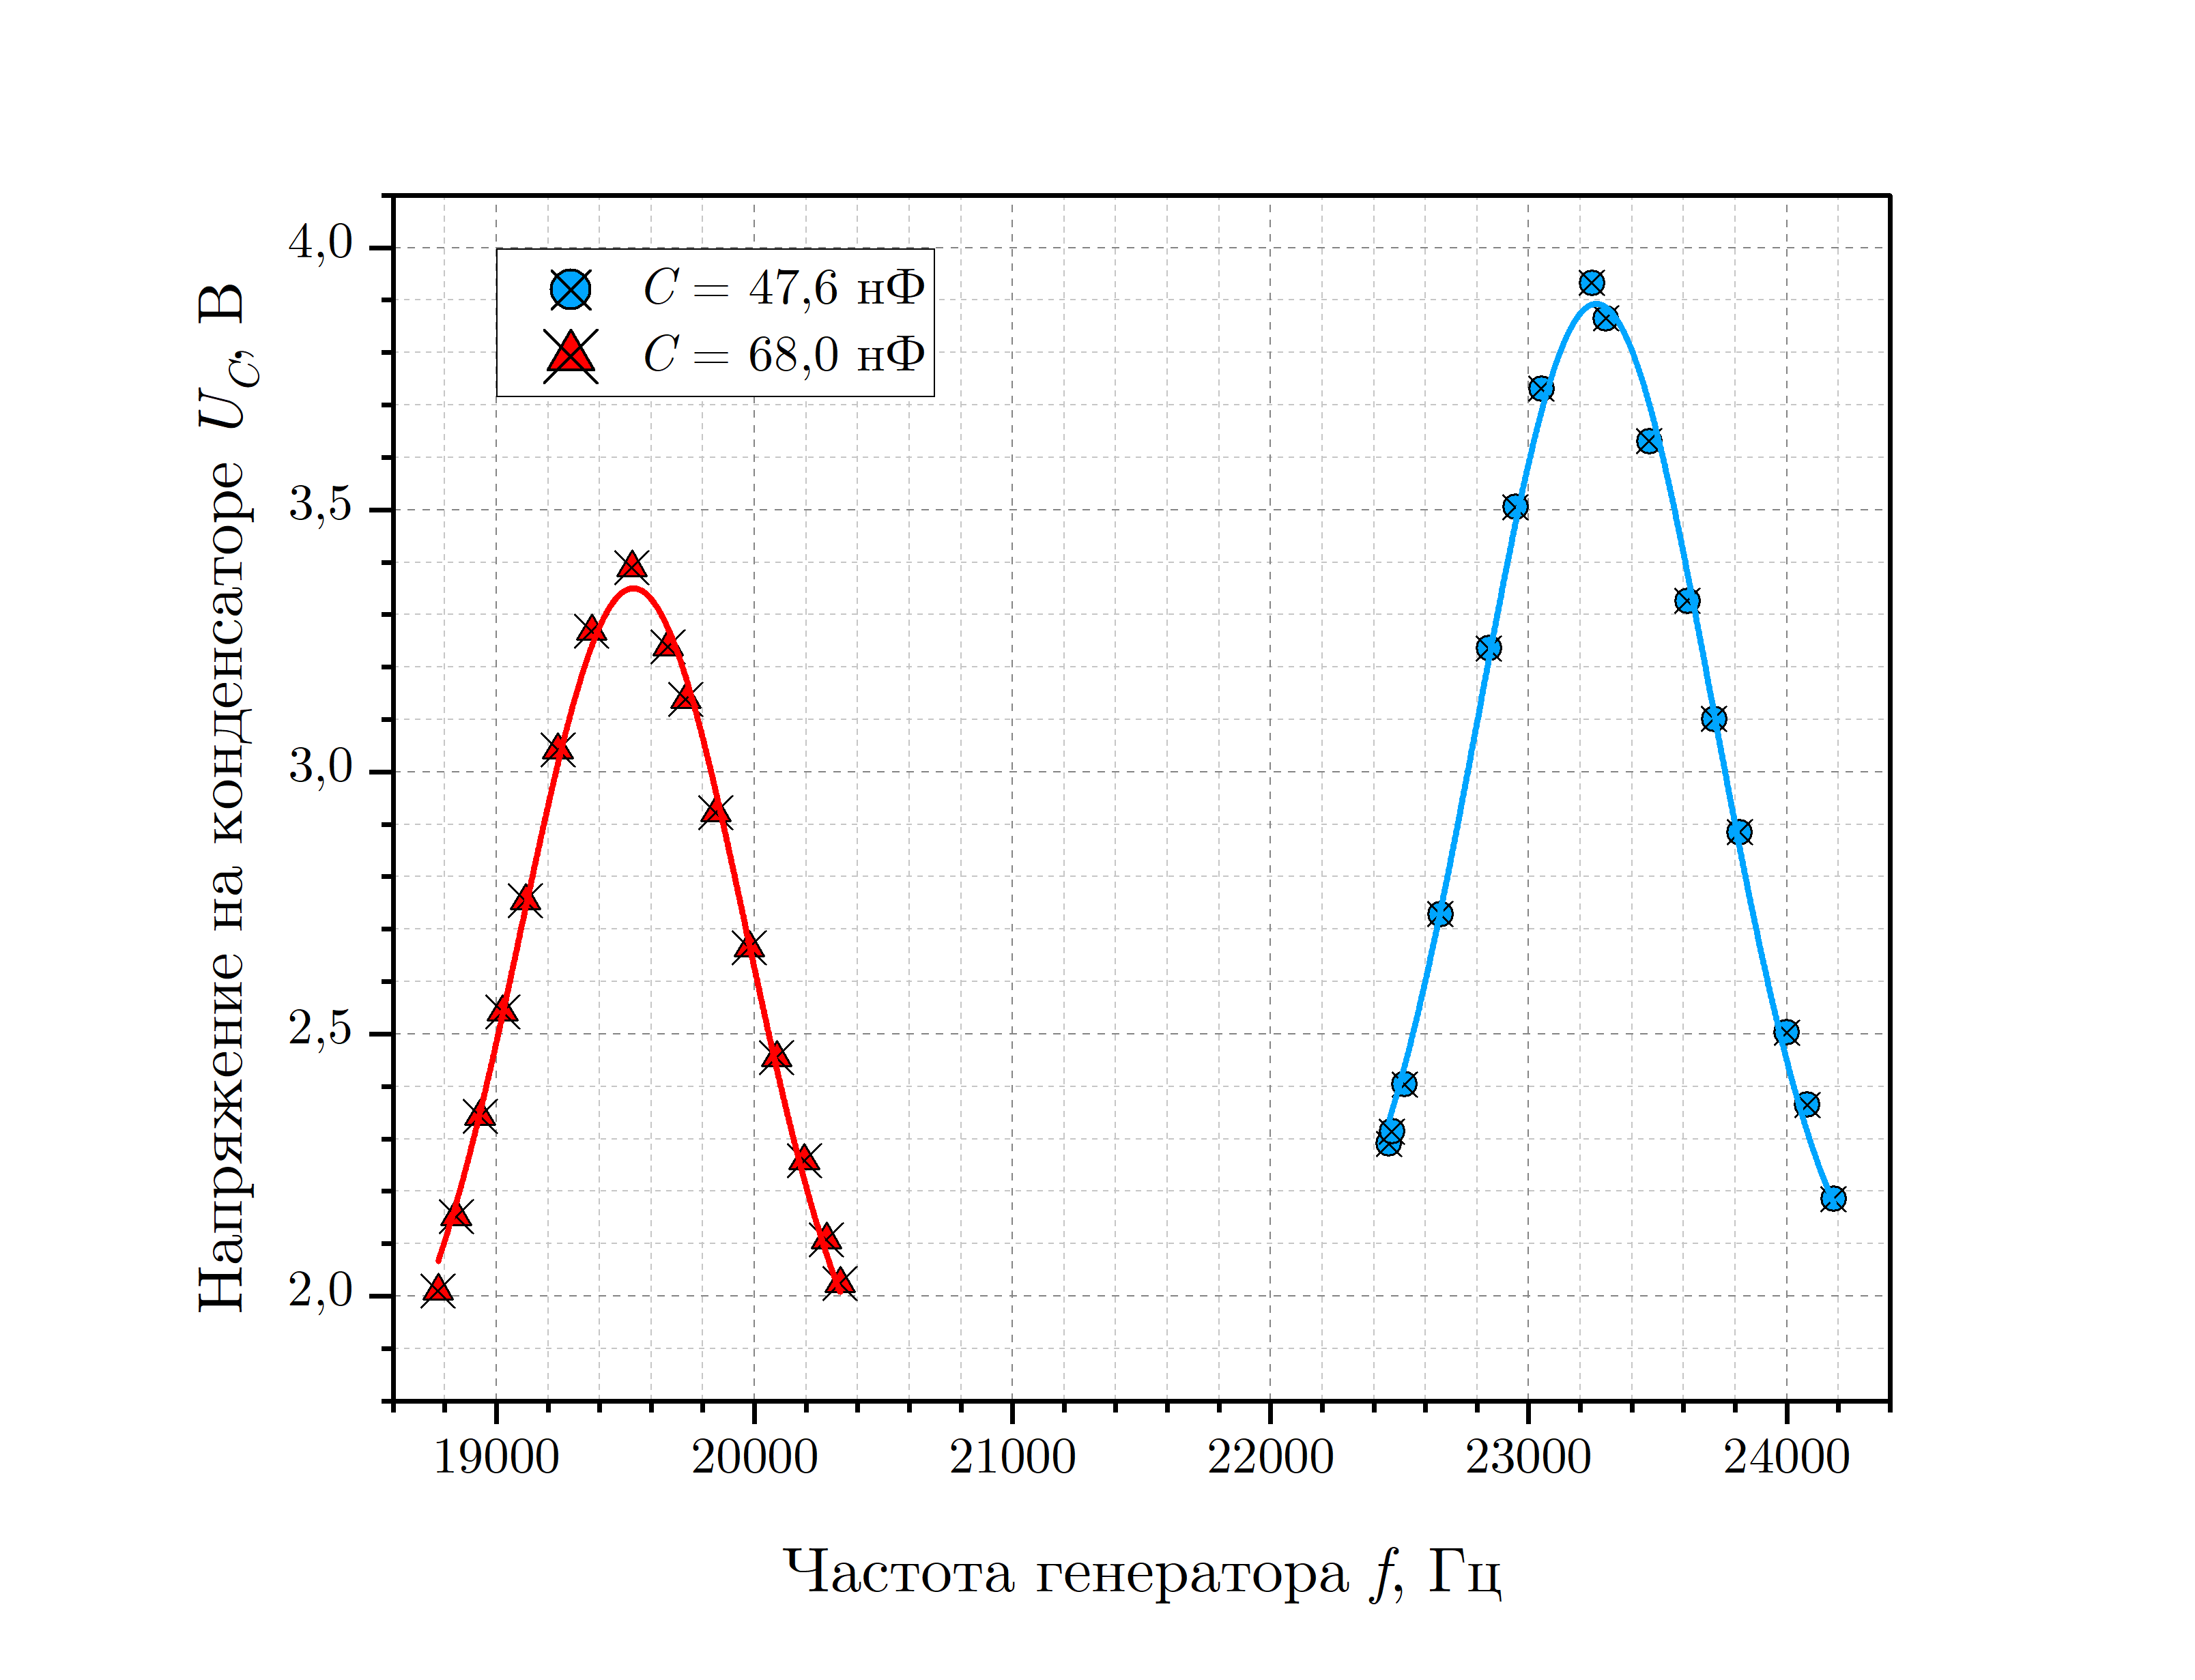
\includegraphics[width = 14cm]{images/graph_AFC.png}
        \caption{Амплитудно-частотная характеристика $U_C(f)$}
        \label{graph_AFC}
    \end{figure}

    Из графика (рис. \ref{graph_AFC}) видно, что резонансная частота и добротность в контуре при $С = 68,0$ нФ меньше. 

    По таблице \ref{tab:res_AFC} также на одном графике были построены амплитудно-частотные характеристики в безразмерных координатах $x = f/f_0$, $y = U_C/U_0$ (рис. \ref{graph_AFC_unit}).

    \begin{figure}[H]
        \centering
        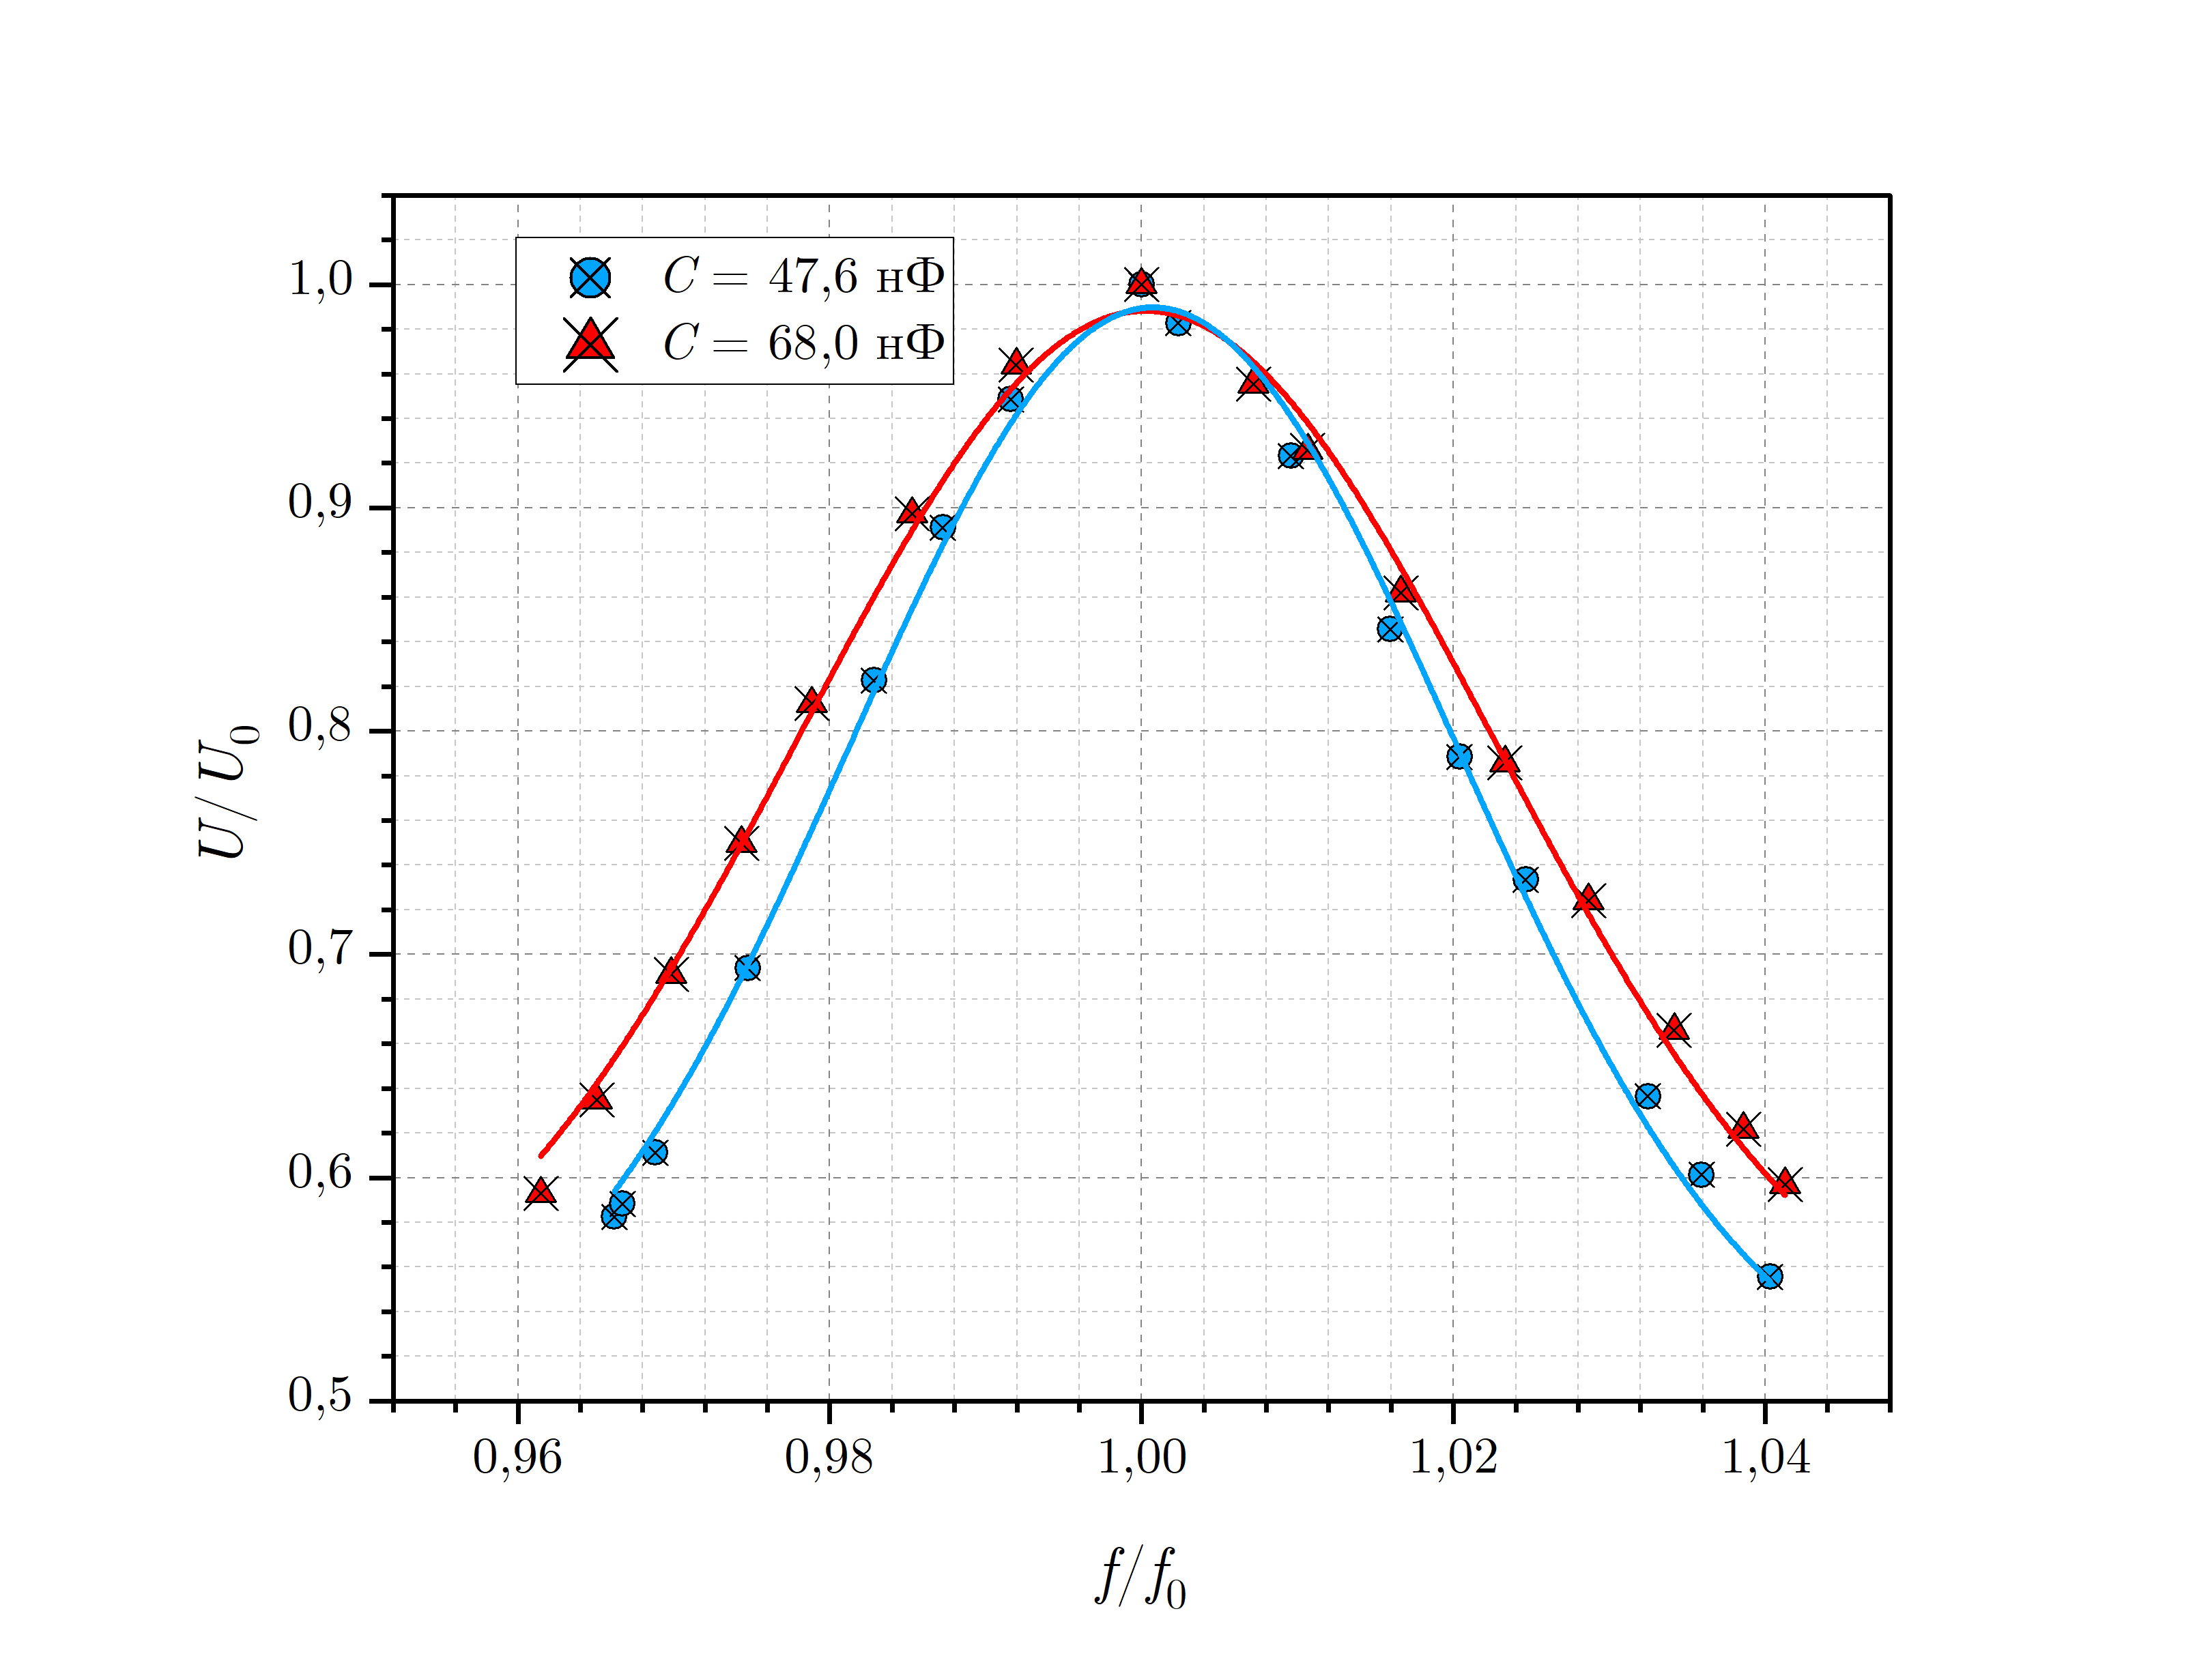
\includegraphics[width = 14cm]{images/graph_AFC_unit.png}
        \caption{Амплитудно-частотная характеристика в безразмерных координатах $x = f/f_0$, $y = U_C/U_0$}
        \label{graph_AFC_unit}
    \end{figure}
    
    Найдём добротность как обратное к разности частот на уровне 0,707:
    
    \begin{equation}
    	\frac{1}{Q_{C=47,6 \text{ нФ}}} = \left(0,050 \pm 0,001 \right) \Rightarrow Q_{C=47,6 \text{ нФ}} = \left(20,0 \pm 0,4 \right)
    \end{equation}
    
    \begin{equation}
    	\frac{1}{Q_{C=68,0 \text{ нФ}}} = \left(0,059 \pm 0,001 \right) \Rightarrow Q_{C=68,0 \text{ нФ}} = \left(16,9 \pm 0,3 \right)
    \end{equation}

    \subsection{Исследование ФЧХ}

    Для контуров с двумя разными ёмкостями были сняты фазово-частотные характеристики $\varphi_C(f)$. Результаты исследования данной зависимости приведены в таблице \ref{tab:res_PFC}.
        
    \begin{table}[H]
        \centering
        \begin{tabular}{|c|c|c|c|c|c|c|c|c|}
        \cline{1-4} \cline{6-9}
        $C_n$, нФ & $f$, Гц & $f/f_0$ & $\Delta \varphi_C /\pi$ & \multirow{19}{*}{} & $C_n$, нФ & $f$, Гц & $f/f_0$ & $\Delta \varphi_C /\pi$ \\ \cline{1-4} \cline{6-9} 
        \multirow{18}{*}{47,6} & 21323 & 0,9173 & 0,0851 &  & \multirow{18}{*}{68,0} & 17868 & 0,9151 & 0,0893 \\ \cline{2-4} \cline{7-9} 
         & 21515 & 0,9256 & 0,1087 &  &  & 17971 & 0,9204 & 0,1091 \\ \cline{2-4} \cline{7-9} 
         & 21784 & 0,9372 & 0,1087 &  &  & 18200 & 0,9321 & 0,1273 \\ \cline{2-4} \cline{7-9} 
         & 21900 & 0,9421 & 0,1304 &  &  & 18385 & 0,9416 & 0,1482 \\ \cline{2-4} \cline{7-9} 
         & 22094 & 0,9505 & 0,1556 &  &  & 18543 & 0,9497 & 0,1482 \\ \cline{2-4} \cline{7-9} 
         & 22285 & 0,9587 & 0,1556 &  &  & 18634 & 0,9543 & 0,1667 \\ \cline{2-4} \cline{7-9} 
         & 22529 & 0,9692 & 0,2273 &  &  & 18717 & 0,9586 & 0,1887 \\ \cline{2-4} \cline{7-9} 
         & 22705 & 0,9768 & 0,2500 &  &  & 19060 & 0,9761 & 0,2885 \\ \cline{2-4} \cline{7-9} 
         & 22930 & 0,9865 & 0,3182 &  &  & 19170 & 0,9818 & 0,3077 \\ \cline{2-4} \cline{7-9} 
         & 23262 & 1,0007 & 0,5116 &  &  & 19229 & 0,9848 & 0,3462 \\ \cline{2-4} \cline{7-9} 
         & 23604 & 1,0154 & 0,6905 &  &  & 19559 & 1,0017 & 0,5294 \\ \cline{2-4} \cline{7-9} 
         & 23866 & 1,0267 & 0,7381 &  &  & 19709 & 1,0094 & 0,5686 \\ \cline{2-4} \cline{7-9} 
         & 24024 & 1,0335 & 0,7619 &  &  & 19967 & 1,0226 & 0,7000 \\ \cline{2-4} \cline{7-9} 
         & 24303 & 1,0455 & 0,8293 &  &  & 20220 & 1,0355 & 0,7400 \\ \cline{2-4} \cline{7-9} 
         & 24475 & 1,0529 & 0,8537 &  &  & 20494 & 1,0496 & 0,8163 \\ \cline{2-4} \cline{7-9} 
         & 24621 & 1,0592 & 0,8537 &  &  & 20710 & 1,0606 & 0,8542 \\ \cline{2-4} \cline{7-9} 
         & 24950 & 1,0734 & 0,9000 &  &  & 20960 & 1,0734 & 0,8750 \\ \cline{2-4} \cline{7-9} 
         & 25407 & 1,0930 & 0,9487 &  &  & 21141 & 1,0827 & 0,9149 \\ \cline{1-4} \cline{6-9} 
        \end{tabular}
        \caption{Результаты измерения зависимости фазово-частотных характеристик}
        \label{tab:res_PFC}
    \end{table}

     По таблице \ref{tab:res_PFC} на одном графике были построены фазово-частотные характеристики в безразмерных координатах $x = f/f_0$, $y = \varphi_C/\pi$ (рис. \ref{graph_PFC_unit}).

    Из графика (рис. \ref{graph_PFC_unit}) видно, что резонансная частота и добротность в контуре при $С = 68,0$ нФ меньше.

    \begin{figure}[H]
        \centering
        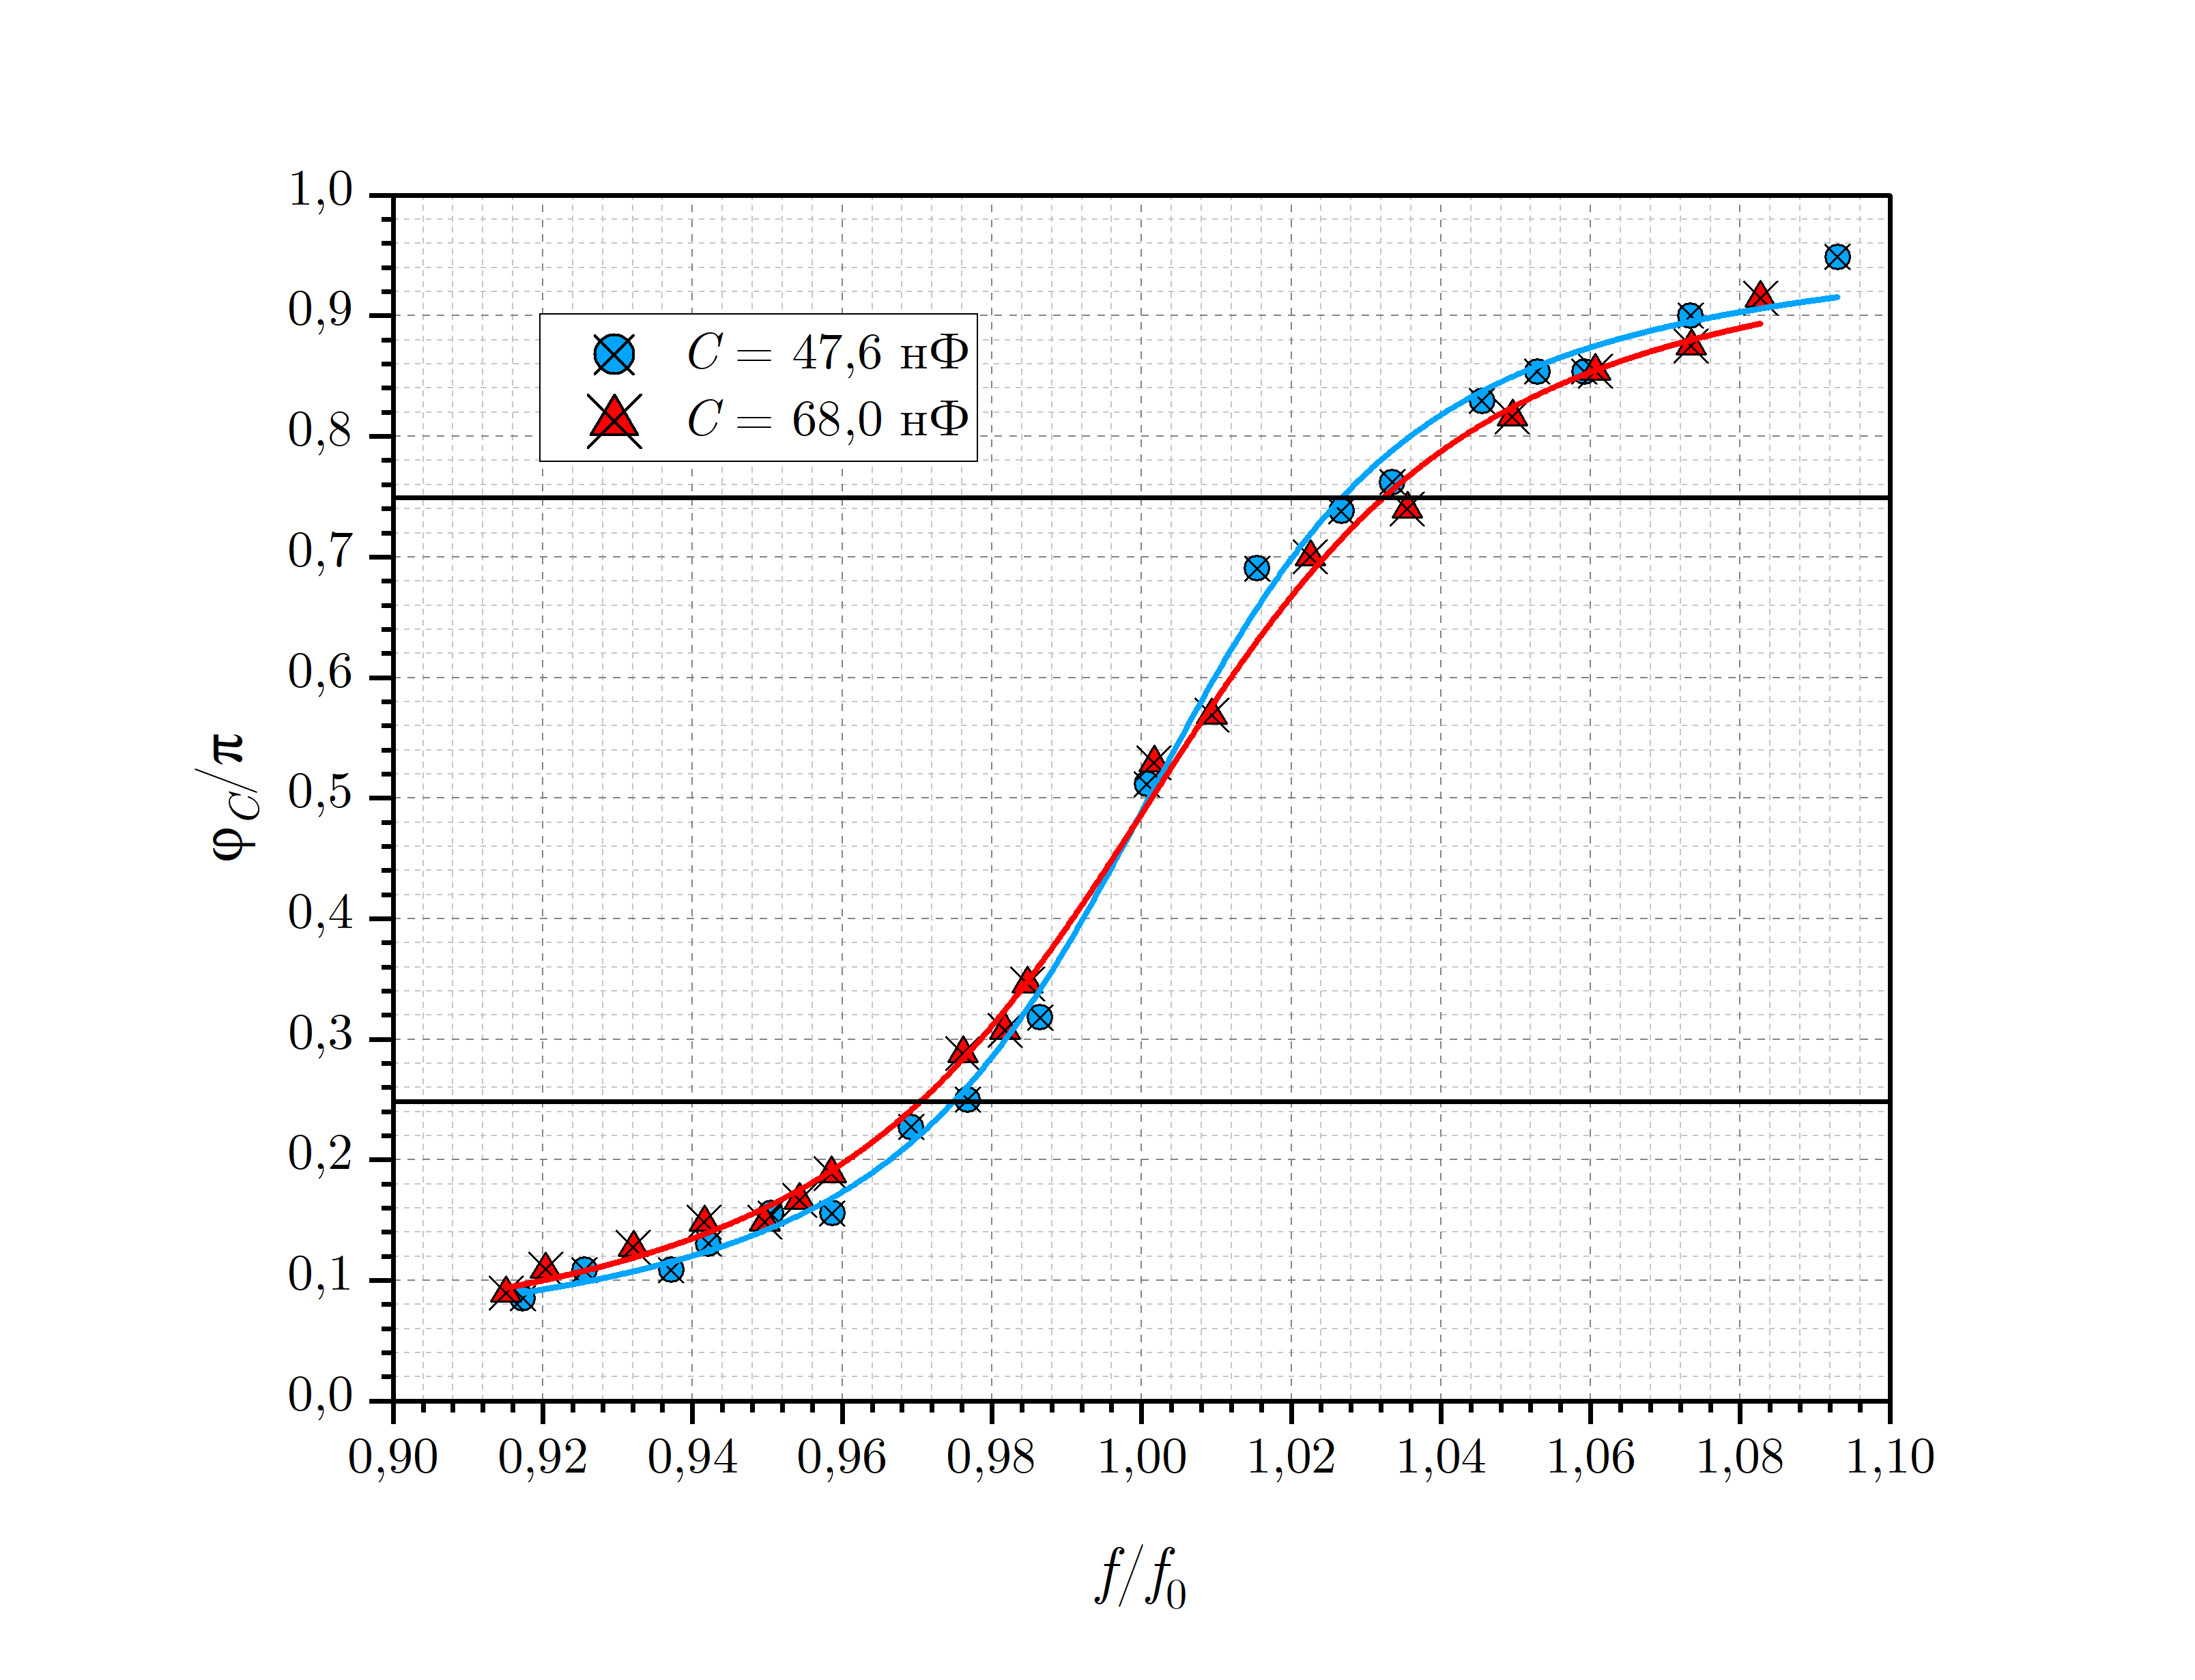
\includegraphics[width = 14cm]{images/graph_PFC_unit.png}
        \caption{Фазово-частотная характеристика в безразмерных координатах $x = f/f_0$, $y = \varphi_C/\pi$}
        \label{graph_PFC_unit}
    \end{figure}
    
    Определим добротность из расстояния по оси $x$ между пересечением графиками прямых $y = 0,25$ и $y = 0,75$:
    
    \begin{equation}
    	\frac{1}{Q_{C=47,6 \text{ нФ}}} = \left(0,050 \pm 0,001 \right) \Rightarrow Q_{C=47,6 \text{ нФ}} = \left(20,0 \pm 0,4 \right)
    \end{equation}
    
    \begin{equation}
    	\frac{1}{Q_{C=68,0 \text{ нФ}}} = \left(0,061 \pm 0,001 \right) \Rightarrow Q_{C=68,0 \text{ нФ}} = \left(16,4 \pm 0,3 \right)
    \end{equation}
    
    \section{Заключение}

    Проведено исследование колебаний напряжения в последовательном контуре. Несколькими методами была определена добротность контуров. Результаты согласуются друг с другом с учётом погрешностей.

    \begin{thebibliography}{9}
        \bibitem{Phys} Сивухин Д. В. \emph{Общий курс физики. -- Т. III. -- Электричество}, 2007
        \bibitem{Lab} Лабораторный практикум по общей физике. -- \emph{Т. II. -- Электричество и магнетизм}, 2019
    \end{thebibliography}

\end{document}